%% ===========================================================================
%%  main.tex — Archivo maestro del paper (IEEE, dos columnas, en inglés)
%%
%%  Efficiency of Asynchronous Dynamic Application Security Testing (DAST):
%%  Payload Scheduling, Runtime Confirmation, and LLM-Based Triage for
%%  False-Positive Reduction.
%%
%%  Estructura modular: cada sección vive en sections/ y se incluye aquí
%%  vía \input{}. Ver README.md.
%%
%%  Compilación (todo en espacio de usuario; nada se escribe en /):
%%      cd paper/submission/
%%      tectonic -X compile main.tex --outdir build --keep-logs
%%  o, con una instalación completa de TeX Live:
%%      latexmk -pdf -output-directory=build main.tex
%% ===========================================================================
\documentclass[conference]{IEEEtran}
\IEEEoverridecommandlockouts

% --- Idioma y codificación ---------------------------------------------------
% inputenc/fontenc solo hacen falta con pdfLaTeX; un motor Unicode
% (XeLaTeX / LuaLaTeX / Tectonic) ya acepta entrada UTF-8 de forma nativa.
\usepackage{iftex}
\ifPDFTeX
  \usepackage[utf8]{inputenc}
  \usepackage[T1]{fontenc}
\fi
\usepackage[english]{babel}
\usepackage{lmodern}
\usepackage{microtype}

% --- Matemáticas, tablas, figuras --------------------------------------------
\usepackage{amsmath,amssymb}
\usepackage{booktabs}
\usepackage{multirow}
\usepackage{siunitx}
\sisetup{detect-weight=true, detect-family=true}
\usepackage{graphicx}
\graphicspath{{figures/}{build/}}
\usepackage{xcolor}

% --- Diagramas ----------------------------------------------------------------
\usepackage{tikz}
\usetikzlibrary{arrows.meta,positioning,fit,backgrounds,calc,shapes.geometric}

% --- Hipervínculos y referencias cruzadas (cargar al final) -----------------
\usepackage[hidelinks,breaklinks]{hyperref}
\usepackage{cleveref}

% --- Ayudas de escritura reutilizables por todos los módulos -----------------
\usepackage{xspace}
\newcommand{\herramienta}{\textsc{WebSecurityScanner}\xspace}
\newcommand{\code}[1]{\texttt{\small #1}}
\newcommand{\rid}{\code{run\_id}\xspace}

% --- Variables de resultados (auto-generadas desde el análisis) ------------
% Todo valor numérico de la Sección 4 vive en este archivo; ver su cabecera.
%% _datos.tex — Macros de variables de resultado, auto-reemplazables desde el análisis.
%%
%%  Fuente: tools/analyze_results.py sobre testbed/experiment_results.csv
%%  (20 corridas de ablación calificadas: presupuestos {10,20,50,inf} x 5
%%  configuraciones de pipeline, todos bloques completos; más 4 corridas
%%  ai-triage, una por presupuesto, evaluadas por separado). Regenerado
%%  2026-09-23 a partir de un barrido de telemetría real contra el banco de
%%  pruebas OWASP Benchmark en vivo.
%%
%%  Convención: los porcentajes incluyen "\%"; las estadísticas usan \num{}.
%%  Salvo que se indique lo contrario, los valores de recall/AUC/costo
%%  corresponden al presupuesto intermedio de 20 peticiones/parámetro (donde
%%  las configuraciones divergen; en presupuestos mayores convergen).

% --- Parámetros fijos del experimento ---------------------------------------
\newcommand{\NumObjetivos}{338}
\newcommand{\NumVulnerables}{194}
\newcommand{\NumTrampas}{144}
\newcommand{\NumCorridas}{20}
\newcommand{\NumConfigsAblation}{5}
\newcommand{\NumBloquesCompletos}{4}
\newcommand{\UmbralTiempo}{4\,s}

% --- Recall en presupuesto 10 y en saturación (presupuesto >= 20) ----------
\newcommand{\ValorRecallBudgetTen}{\num{0.675}}
\newcommand{\ValorRecallTecho}{\num{70.6}\%}

% --- Área bajo la curva de detección (AUC = recall medio / presupuesto) ----
% En el presupuesto intermedio de 20 peticiones/parámetro:
\newcommand{\ValorAUCBaseline}{\num{0.356}}
\newcommand{\ValorAUCNoInterleave}{\num{0.356}}
\newcommand{\ValorAUCNoPriority}{\num{0.350}}
\newcommand{\ValorAUCNoRuntimeConfirm}{\num{0.355}}
\newcommand{\ValorAUCNoAdaptiveSorting}{\num{0.355}}
% El AUC por presupuesto y Prec./Rec./F1 de las cinco configuraciones están
% escritos directamente en las columnas S de la Tabla tab:auc (las columnas S
% de siunitx rechazan macros \num{} anidadas), tomados de
% testbed/analysis/summary_by_run.csv.

% --- Métricas agregadas de baseline (presupuesto 20) ------------------------
\newcommand{\ValorPrecisionBaseline}{\num{64.0}\%}
\newcommand{\ValorRecallBaseline}{\num{70.6}\%}
\newcommand{\ValorFOneBaseline}{\num{67.2}\%}
\newcommand{\ValorFPRBaseline}{\num{1.4}\%}
\newcommand{\ValorFPRBudgetAlto}{\num{2.1}\%}

% --- Caída de recall/precisión al desactivar cada optimización vs. baseline,
%     en presupuesto 20 (puntos porcentuales) -------------------------------
\newcommand{\DeltaRecallNoInterleave}{\num{0.0}~p.p.}
\newcommand{\DeltaRecallNoPriority}{\num{3.1}~p.p.}
\newcommand{\DeltaRecallNoRuntimeConfirm}{\num{0.0}~p.p.}
\newcommand{\DeltaPrecisionNoPriority}{\num{5.5}~p.p.}
\newcommand{\DeltaFOneNoPriority}{\num{4.5}~p.p.}
\newcommand{\NoPriorityVulnPerdidas}{6}
\newcommand{\NoPriorityFPnuevos}{16}

% --- Costo medio de detección (índice del primer hallazgo, censurado; bloque agrupado) -
\newcommand{\ValorCosteBaseline}{\num{40247}}
\newcommand{\ValorCosteNoInterleave}{\num{40042}}
\newcommand{\ValorCosteNoPriority}{\num{39847}}
\newcommand{\ValorCosteNoRuntimeConfirm}{\num{40226}}

% --- Test de Friedman sobre costo de detección por instancia, bloque agrupado
%     de los 4 presupuestos completos {10,20,50,inf} ------------------------
\newcommand{\ValorFriedmanChiSq}{\num{1001.7}}
\newcommand{\ValorFriedmanP}{\num{7.8e-217}}
\newcommand{\ValorFriedmanN}{\num{776}}

% --- Wilcoxon pareado (baseline vs. ablación), p corregido BH (agrupado) ---
\newcommand{\ValorWilcoxonPNoInterleave}{\num{9.1e-31}}
\newcommand{\ValorWilcoxonPNoPriority}{\num{4.4e-103}}
\newcommand{\ValorWilcoxonPNoRuntimeConfirm}{\num{3.6e-4}}

% --- Tamaño del efecto: delta de Cliff (baseline vs. ablación, agrupado) ---
\newcommand{\ValorCliffNoInterleave}{\num{-0.001}}
\newcommand{\ValorCliffNoPriority}{\num{-0.012}}
\newcommand{\ValorCliffNoRuntimeConfirm}{\num{-0.001}}
\newcommand{\MagnitudCliffNoInterleave}{negligible}
\newcommand{\MagnitudCliffNoPriority}{negligible}
\newcommand{\MagnitudCliffNoRuntimeConfirm}{negligible}

% --- Nemenyi post-hoc (agrupado): p de baseline vs. cada ablación ----------
\newcommand{\ValorNemenyiNoInterleave}{\ensuremath{<}\,\num{0.001}}
\newcommand{\ValorNemenyiNoPriority}{\ensuremath{<}\,\num{0.001}}
\newcommand{\ValorNemenyiNoRuntimeConfirm}{\num{0.361}}

% --- Brazo de triaje LLM (ai-triage): candidatos totales en los 4
%     presupuestos y traza de auditoría por presupuesto (filas 50 / ilimitado
%     referenciadas en la Tabla tab:aitriage; 10 / 20 van directo en el texto
%     de sec:ai-triage-result) --------------------------------------------
\newcommand{\ValorAITriageTotalTriaged}{\num{1852}}
\newcommand{\ValorAITriageBudgetFiftyTriaged}{476}
\newcommand{\ValorAITriageBudgetFiftySuppressed}{0}
\newcommand{\ValorAITriageBudgetFiftyFPSuppressed}{0}
\newcommand{\ValorAITriageBudgetFiftyFNIntroduced}{0}
\newcommand{\ValorAITriageBudgetInfTriaged}{476}
\newcommand{\ValorAITriageBudgetInfSuppressed}{0}
\newcommand{\ValorAITriageBudgetInfFPSuppressed}{0}
\newcommand{\ValorAITriageBudgetInfFNIntroduced}{0}


% Estilos de bloque para el diagrama TikZ de arquitectura.
\tikzset{
  bloque/.style    = {rectangle, rounded corners=2pt, draw=black!70,
                      fill=black!4, align=center, font=\footnotesize,
                      minimum height=8mm, inner sep=3pt},
  nucleo/.style    = {bloque, fill=blue!8,   draw=blue!55},
  ablac/.style     = {bloque, fill=orange!12, draw=orange!60},
  artefacto/.style = {bloque, fill=green!9,  draw=green!55},
  flecha/.style    = {-{Stealth[length=2mm]}, thick, draw=black!65},
}

% ===========================================================================
\begin{document}

%% 00_abstract.tex — Título, autoría, resumen, palabras clave.

\title{Efficiency of Asynchronous Dynamic Application Security Testing:\\
Payload Scheduling, Runtime Confirmation, and LLM-Based Triage\\
for False-Positive Reduction}

\author{%
\IEEEauthorblockN{Luis Ernesto Gald\'amez Vides}
\IEEEauthorblockA{%
Universidad Evang\'elica de El Salvador (UEES)\\
San Salvador, El Salvador\\
\texttt{2026010235@cvirtualuees.edu.sv}%
}
}

\maketitle

\begin{abstract}
Dynamic Application Security Testing (DAST) scanners are widely used in
continuous-integration pipelines, but their practical adoption is limited by
three factors: the accumulated latency of thousands of sequential requests,
the noise produced by a high false-positive rate, and the combinatorial
explosion of the payload space per injection point. This paper presents and
evaluates \herramienta, a DAST engine built entirely on \code{asyncio} that
introduces (i)~a payload-scheduling pipeline --- context interleaving,
a-priori confidence prioritization, and configurable ordering, including a
live adaptive-sorting feedback loop --- (ii)~a runtime-confirmation stage that
relabels every finding with a calibrated confidence level before it is
reported, and (iii)~an optional LLM-based triage stage that re-scores each raw
finding using request/response context, without an additional network round
trip to the target. The central hypothesis is that
these techniques improve the detection-to-cost ratio (number of requests)
without increasing the false-positive rate. To test it we built a reproducible
testbed on OWASP Benchmark restricted to \num{338}~\code{GET}-parameter
targets (\num{194}~vulnerable instances and \num{144}~known traps), an
ablation study under a randomized complete block design (RCBD) with four
request budgets and six pipeline configurations, and a battery of
non-parametric tests (Friedman, Nemenyi post-hoc, paired Wilcoxon with
Benjamini--Hochberg correction, and Cliff's $\delta$ as effect size).
Reproducibility is guaranteed through a per-run manifest that fixes the
SHA-256 hash of the payload corpus, the \code{git} commit, and the global seed
of the random-number generator. The full heuristic pipeline reaches
\ValorRecallTecho{} recall at a \ValorFPRBaseline{} false-positive rate and
already saturates at \num{20}~requests per parameter. Of the three
heuristic-pipeline optimizations, only confidence-based prioritization has a
practically consequential effect --- and it is bounded to tight budgets:
context interleaving and runtime confirmation shift the request order in a
statistically detectable way (Friedman, $p \ll 0.001$) but with negligible
effect sizes ($\lvert\delta\rvert < 0.02$). Layering LLM-based triage on top
of the baseline pipeline, evaluated separately across the same budget grid,
suppressed \emph{zero} findings at every budget under its default confidence
threshold, adding no measurable wall-clock overhead to the scan; we report
this null result openly and attribute it to the benchmark's unusually
unambiguous trigger signals rather than to the triage stage being validated
as safe or effective in general. Run against OWASP ZAP 2.17.0 on the
identical target list under the same oracle, \code{baseline} matches ZAP's
recall exactly (both detect the same \num{137}/\num{194} instances), at the
cost of a higher false-positive rate on the known traps (ZAP: \num{0}\,\%).
It reaches that recall \num{11}$\times$ faster than ZAP at its saturating
budget. We conclude that, on a benchmark with regular trigger signals, the
value of payload scheduling is one of \emph{anticipation} (higher AUC under
a tight budget), not of a higher detection ceiling. The LLM-triage stage
remains to be stress-tested on a noisier target.
\end{abstract}

\begin{IEEEkeywords}
web application security, DAST, dynamic analysis, asynchronous programming,
false positives, payload scheduling, LLM triage, reproducible evaluation,
OWASP Benchmark.
\end{IEEEkeywords}

%% 01_introduccion.tex — Contexto, retos, trabajo relacionado, contribuciones.

\section{Introduction}
\label{sec:intro}

Dynamic Application Security Testing (DAST) evaluates a running system by
sending manipulated requests and observing the response, with no access to
source code. Compared to static analysis, its main advantage is the absence
of assumptions about the target's language or framework; its main drawback is
cost. Comparative studies have repeatedly shown that black-box scanners
exhibit uneven coverage and elevated false-positive
rates~\cite{doupe2010johnny,bau2010state,parvez2015analysis}, which erodes the
development team's trust and, in practice, leads reports to be ignored.

We identify three concrete challenges that this work addresses explicitly:

\begin{enumerate}
  \item \textbf{Accumulated latency.} A realistic scan involves on the order
  of $10^4$--$10^5$ HTTP requests. Executed sequentially, network latency
  dominates total run time and makes integrating DAST into every \emph{commit}
  infeasible.
  \item \textbf{Noise (false positives).} Detection based solely on a
  reflected string or a database error pattern produces findings that are not
  exploitable. Telling an inert reflection apart from real execution requires
  a second, targeted observation.
  \item \textbf{Combinatorial explosion.} The product (injection points)
  $\times$ (payloads per category) $\times$ (evasion transformations) grows
  until testing everything under a fixed time budget becomes impossible; the
  order in which that budget is spent determines what gets detected. This
  paper's architecture is designed to withstand that growth (\cref{sec:pipeline}),
  but the evaluation in \cref{sec:resultados} exercises the scheduling
  mechanics on a constrained corpus --- \num{338}~\code{GET} parameters that
  saturate at \num{20}~requests each --- not a payload space large enough to
  demonstrate the explosion itself; \cref{sec:amenazas} discusses this
  restriction.
\end{enumerate}

\subsection{Related work}
\label{sec:related}

\noindent\textbf{LLM-based vulnerability triage.} LLM-assisted triage of
security findings is an active area outside of DAST. Static-analysis
pipelines that pair a deterministic scanner (Semgrep, CodeQL) with an LLM
adjudication stage report large false-positive reductions: Munson~\emph{et
al.} enrich static findings with reachability context before LLM
adjudication~\cite{munson2025llmfriends}; Ameen~\emph{et al.}'s multi-agent
\textsc{QASecClaw} raises the $F_1$ score of standalone Semgrep from
78.4\,\% to 90.9\,\% on Java test cases by suppressing non-exploitable
alerts~\cite{ameen2026qasecclaw}; Agrawal and Ahi's \textsc{SAST-Genius}
hybrid framework cuts Semgrep's false positives by 91\,\% (225 to 20) through
LLM-driven triage, dynamic bug descriptions, and exploit-generation
validation~\cite{agrawal2025sastgenius}; and Du~\emph{et al.}'s industrial
study at Tencent reports that hybrid LLM/static-analysis triage eliminates
94--98\,\% of false positives while preserving recall, at a marginal cost of
\SIrange{2.1}{109.5}{\second} per alert~\cite{du2026reducing}. These results
motivate the LLM-triage stage evaluated in \cref{sec:ai-triage}: unlike the
static-analysis setting, a DAST finding already carries live request/response
evidence, so triage here re-scores an executed probe rather than a static
alert. All four studies report their false-positive reductions against
corpora with a substantial false-positive population to begin with; none
addresses the scheduling problem that determines \emph{which} payloads reach
the target under a fixed request budget in the first place, nor evaluates
triage on a target whose noise floor is already low --- both of which
\cref{sec:resultados,sec:ai-triage} take up directly.

\noindent\textbf{Payload and seed scheduling.} Outside DAST, the greybox
fuzzing literature treats seed/input scheduling as a first-class problem:
She~\emph{et al.} prioritize fuzzing seeds by graph-centrality analysis of
the program's control-flow graph to maximize coverage growth per
execution~\cite{she2022effective}, the same anticipation argument this paper
makes for confidence-based payload prioritization
(\cref{sec:pipeline,sec:res-sintesis}) --- earlier detection per request
under a fixed budget, not necessarily a higher final yield. To our knowledge
no prior work transfers this scheduling framing to black-box DAST payload
selection, where the search space is a fixed, tester-supplied corpus rather
than a mutation-generated one.

\noindent\textbf{OWASP Benchmark as an evaluation target.} Potti~\emph{et
al.} benchmark OWASP ZAP v2.12.0 and v2.13.0 on the OWASP Benchmark project,
reporting an aggregate true-positive rate of 68.75--74.63\,\% at a
0.86--3.45\,\% false-positive rate across vulnerability
categories~\cite{potti2025benchmarking}. \Cref{sec:res-external} runs a newer
ZAP release (2.17.0) ourselves against this paper's own \num{338}-target
list under the same oracle used throughout this paper, and finds their
published range consistent with our own single-run result.

\noindent\textbf{Contributions.} This paper makes the following
contributions:

\begin{itemize}
  \item An asynchronous DAST engine with a single HTTP choke point,
  back-pressured concurrency control, token-bucket rate limiting, and
  safeguards against SSRF in redirect following (\cref{sec:arquitectura}).
  \item A payload-scheduling pipeline with decoupled stages --- context
  interleaving, prioritization, ordering, and a live adaptive-sorting
  feedback loop --- plus a runtime-confirmation stage that calibrates finding
  confidence (\cref{sec:arquitectura,sec:metodologia}).
  \item An optional LLM-based triage stage that re-scores executed probes
  using request/response context, and an honest evaluation of it against the
  same budget grid, including a null-result case where it suppresses nothing
  and a measured wall-clock overhead of zero (\cref{sec:ai-triage}).
  \item A non-blocking \code{TelemetryWorker} that logs one JSONL row per
  payload probe, enabling instance-by-instance detection-cost measurement
  (\cref{sec:telemetria}).
  \item A reproducible evaluation methodology: a containerized testbed, an
  independent grading oracle, an RCBD experimental design, and a
  reproducibility manifest with a corpus hash (\cref{sec:metodologia}).
  \item An ablation study that isolates each pipeline stage's contribution to
  the detection-versus-cost curve and to the false-positive rate
  (\cref{sec:resultados}).
  \item An external baseline against OWASP ZAP on the identical target list
  under the same oracle, reported honestly including the categories where
  ZAP outperforms \herramienta (\cref{sec:res-external}).
\end{itemize}

The rest of the paper is organized as follows. \Cref{sec:arquitectura}
describes the engine's design. \Cref{sec:metodologia} details the testbed and
the experimental design. \Cref{sec:resultados} presents the ablation
evaluation and \cref{sec:ai-triage} the LLM-triage evaluation.
\Cref{sec:amenazas} discusses threats to validity, and \cref{sec:conclusion}
concludes.

%% 02_arquitectura.tex — Motor asíncrono, pipeline de ablación, telemetría.

\section{Architecture and Design}
\label{sec:arquitectura}

\herramienta is structured into four subsystems: the asynchronous HTTP core,
the payload loader, the vulnerability-tester hierarchy with its scheduling
pipeline, and the telemetry/reproducibility instrumentation.
\Cref{fig:arquitectura} summarizes the workflow.

% ---------------------------------------------------------------- figura ----
\begin{figure*}[t]
  \centering
  \resizebox{\textwidth}{!}{%
  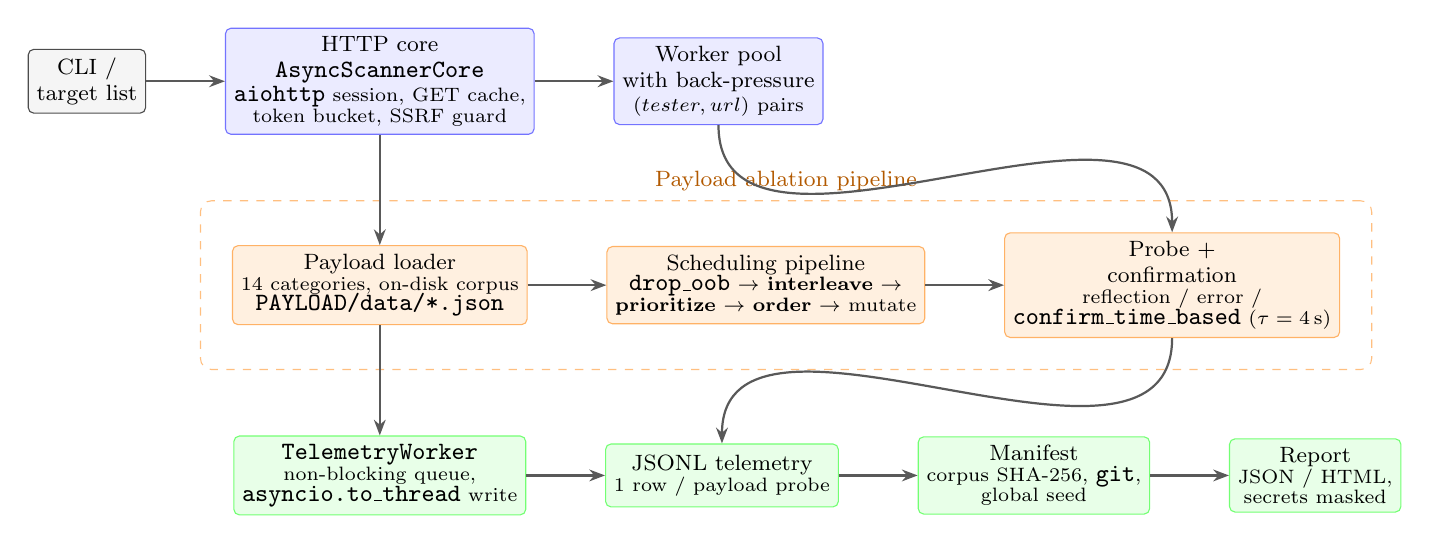
\begin{tikzpicture}[node distance=6mm and 10mm]
    % --- entrada
    \node[bloque] (cli) {CLI / \\ target list};
    \node[nucleo, right=of cli] (core) {HTTP core \\ \code{AsyncScannerCore}\\[-1pt]
      \scriptsize \code{aiohttp} session, GET cache,\\[-2pt]
      \scriptsize token bucket, SSRF guard};
    \node[nucleo, right=of core] (pool) {Worker pool \\ with back-pressure\\[-1pt]
      \scriptsize $(tester, url)$ pairs};

    % --- pipeline de ablación
    \node[ablac, below=14mm of core] (load) {Payload loader\\[-2pt]
      \scriptsize 14 categories, on-disk corpus\\[-2pt]
      \scriptsize \code{PAYLOAD/data/*.json}};
    \node[ablac, right=of load] (sched) {Scheduling pipeline\\[-2pt]
      \scriptsize \code{drop\_oob} $\to$ \textbf{interleave} $\to$\\[-2pt]
      \scriptsize \textbf{prioritize} $\to$ \textbf{order} $\to$ mutate};
    \node[ablac, right=of sched] (probe) {Probe + \\ confirmation\\[-2pt]
      \scriptsize reflection / error / \\[-2pt]
      \scriptsize \code{confirm\_time\_based} ($\tau=\SI{4}{\second}$)};

    % --- artefactos
    \node[artefacto, below=14mm of load] (tel) {\code{TelemetryWorker}\\[-2pt]
      \scriptsize non-blocking queue,\\[-2pt]
      \scriptsize \code{asyncio.to\_thread} write};
    \node[artefacto, right=of tel] (jsonl) {JSONL telemetry\\[-2pt]
      \scriptsize 1 row / payload probe};
    \node[artefacto, right=of jsonl] (manif) {Manifest\\[-2pt]
      \scriptsize corpus SHA-256, \code{git},\\[-2pt]
      \scriptsize global seed};
    \node[artefacto, right=of manif] (report) {Report\\[-2pt]
      \scriptsize JSON / HTML,\\[-2pt]
      \scriptsize secrets masked};

    % --- flechas
    \draw[flecha] (cli) -- (core);
    \draw[flecha] (core) -- (pool);
    \draw[flecha] (pool.south) to[out=-90,in=90] (probe.north);
    \draw[flecha] (load) -- (sched);
    \draw[flecha] (sched) -- (probe);
    \draw[flecha] (core.south) to[out=-90,in=90] (load.north);
    \draw[flecha] (probe.south) to[out=-90,in=90] (jsonl.north);
    \draw[flecha] (load.south) to[out=-90,in=90] (tel.north);
    \draw[flecha] (tel) -- (jsonl);
    \draw[flecha] (jsonl) -- (manif);
    \draw[flecha] (manif) -- (report);

    \begin{scope}[on background layer]
      \node[fit=(load)(sched)(probe), draw=orange!50, dashed,
            rounded corners, inner sep=4mm,
            label={[orange!70!black,font=\footnotesize]above:%
            Payload ablation pipeline}] {};
    \end{scope}
  \end{tikzpicture}%
  }
  \caption{Workflow of \herramienta. The asynchronous HTTP core concentrates
  all network I/O; the worker pool dispatches $(tester, url)$ pairs with
  back-pressure. Each tester loads its payload corpus and runs it through the
  scheduling pipeline before probing the target. The confirmation stage
  relabels finding confidence. \code{TelemetryWorker} writes one JSONL row per
  probe without blocking the event loop; the manifest fixes the
  reproducibility inputs.}
  \label{fig:arquitectura}
\end{figure*}

\subsection{Asynchronous HTTP core}
\label{sec:nucleo}

All network traffic goes through \code{AsyncScannerCore.request()}, a single
choke point built on an \code{aiohttp.ClientSession}. Centralizing I/O lets
the engine uniformly apply: (a)~a response cache for \code{200}-status
\code{GET} requests; (b)~token-bucket rate limiting; (c)~seedable User-Agent
rotation; (d)~separate timeouts for connection establishment and socket
reads; (e)~a \SI{5}{\mebi\byte} cap on the response body, with chunked reading
and a truncation flag; and (f)~a Server-Side Request Forgery safeguard that
rejects redirects toward private addresses unless explicitly authorized. The
\code{elapsed} field the core returns is monotonic and spans redirects; for
per-probe latency measured for scientific purposes, \code{time.perf\_counter()}
is instead measured at the tester boundary.

Work dispatch uses \code{run\_worker\_pool()}, which enforces back-pressure
through a bounded queue (\code{queue\_factor}) so that target discovery cannot
overrun memory or saturate the target. \code{SIGINT} handling is orderly: the
queue is drained and the session is closed idempotently.

\subsection{Payload-scheduling pipeline}
\label{sec:pipeline}

Every tester derives from a common base class that resolves payload loading
through \code{load\_payloads()}. Internally, this routine applies, in order,
the following stages, all of them independently toggleable for the ablation
study:

\begin{enumerate}
  \item \code{\_drop\_useless\_oob}: discards out-of-band payloads when no
  collector is configured.
  \item \code{\_interleave\_by\_context} (\textsc{interleave}): reorders the
  list to alternate across syntactic contexts (HTML, attribute, JavaScript,
  URL, SQL, \dots) instead of exhausting one context before moving to the
  next. The intuition is that, under a tight budget, covering one
  representative payload per context first maximizes the probability of an
  early hit.
  \item \code{\_prioritize} (\textsc{prioritize}): a stable sort by
  $(\text{a-priori confidence}, \text{severity})$, so that vectors with higher
  historical success probability and greater impact are tried first.
  \item \code{\_apply\_payload\_order} (\textsc{order}): a configurable
  terminal policy --- \code{natural} (identity), \code{random} (seeded
  shuffle), or \code{freq} (most-populated context groups first).
  \item \textbf{Live adaptive sorting} (\textsc{adaptive}): a
  feedback loop that re-ranks the remaining queue mid-scan using the
  hit/miss outcomes observed so far for each context, in place of the
  a-priori \code{freq} order fixed before the scan starts. Disabling it
  (\code{--no-adaptive-sorting}) pins the pipeline to the static a-priori
  order and isolates the contribution of the online feedback loop
  (\cref{sec:resultados}).
  \item \code{\_apply\_runtime\_mutations}: WAF-evasion transformations and
  case variation applied at send time.
\end{enumerate}

\subsection{Runtime confirmation and calibrated confidence}
\label{sec:confirmacion}

Every finding carries a confidence level from the ordered domain
$\{\textsc{low}, \textsc{medium}, \textsc{high}, \textsc{confirmed}\}$. The
corpus assigns an a-priori confidence to each payload; the confirmation stage
produces the \emph{final} confidence:

\begin{itemize}
  \item \textbf{Time-based SQL injection.} Baseline latency is resampled
  (\code{measure\_baseline\_latency}) and the response to the timed payload is
  contrasted against a threshold $\tau = \SI{4}{\second}$
  (\code{confirm\_time\_based}); only if the difference exceeds the threshold
  is the finding marked \textsc{confirmed}.
  \item \textbf{XSS.} A raw reflection is refined according to the HTML
  context in which it appears (\code{\_assess}), promoting it to \textsc{high}
  or downgrading it to \textsc{low}.
  \item Under the \code{--no-runtime-confirm} ablation, both branches are
  short-circuited and the finding is reported with the payload's a-priori
  confidence, leaving a record (\code{verification=skipped}) in the evidence.
  The probe is logged to telemetry either way.
\end{itemize}

\subsection{Non-blocking telemetry}
\label{sec:telemetria}

\code{TelemetryWorker} decouples event generation from persistence. Its
\code{record()} method is synchronous and non-blocking: it enqueues the row
and assigns a \code{request\_index} (run-scoped, monotonic), an ISO-8601 UTC
timestamp, and a \rid. An asynchronous consumer batches rows and writes them
through \code{asyncio.to\_thread()}, so the event loop never blocks on disk
I/O. If the queue fills up, excess rows are dropped and counted
(\code{dropped}), preserving the back-pressure property.

The \textbf{granularity} is deliberate: one JSONL row per \emph{payload
probe}, after the tester's confirmation heuristics, not per socket write.
Baseline and confirmation sub-requests are not logged individually. Each
row's schema includes \code{run\_id, timestamp, tester\_id, payload\_id,
context, confidence\_apriori, url, method, elapsed\_time, decision,
confidence\_final}, and \code{request\_index}. This trace is the primary input
for the detection-cost analysis in \cref{sec:resultados}.

\subsection{Reproducibility: the per-run manifest}
\label{sec:manifiesto}

Alongside telemetry, every instrumented run emits a JSON manifest that fixes:
the schema version, the \rid, the creation timestamp, the \code{git} commit
(\code{unknown} when not applicable), the RNG's global seed, and a
\code{corpus} block with the SHA-256 hash computed over the sorted
\code{PAYLOAD/data/*.json} files (each file name is mixed into the digest)
plus the file list and its count. The complete run configuration dictionary
is also included. Hash computation and the \code{git} query run on a separate
thread; a failure is logged and ignored, without aborting or delaying the
scan. This artifact makes it possible to verify \emph{a posteriori} that two
runs share exactly the same corpus and configuration.

%% 03_metodologia.tex — Banco de pruebas, oráculo, diseño RCBD, reproducibilidad.

\section{Experimental Methodology}
\label{sec:metodologia}

\subsection{Testbed}
\label{sec:testbed}

The evaluation target is OWASP Benchmark~\cite{owaspbenchmark}, a
deliberately vulnerable Java application with labeled test cases. It is
deployed via \code{docker compose}, serving HTTPS on port \num{8443} with a
self-signed certificate (hence every probe uses \code{-{}-no-verify-ssl}). To
bound the study to a single vector type, the benchmark is restricted to the
\textbf{\num{338}~\code{GET}-parameter cases} (\code{vector = getparam}). The
\code{build\_ground\_truth.py} generator produces the ground-truth file as an
array of
$\langle \code{url}, \code{param}, \code{type}, \code{vulnerable} \rangle$
records; records with \code{vulnerable = false} are explicit \emph{traps}
(known-safe points that must not fire). \Cref{tab:testbed} summarizes its
composition.

\begin{table}[t]
  \centering
  \caption{Ground-truth composition (OWASP Benchmark, \code{getparam}
  vectors).}
  \label{tab:testbed}
  \begin{tabular}{lrr}
    \toprule
    Category & Vulnerable instances & Traps \\
    \midrule
    Reflected XSS            & 68 & \multirow{5}{*}{144} \\
    SQL Injection             & 65 & \\
    Path Traversal            & 30 & \\
    Command Injection         & 25 & \\
    LDAP Injection             & 6  & \\
    \midrule
    \textbf{Total}            & \textbf{194} & \textbf{144} \\
    \bottomrule
  \end{tabular}
\end{table}

\subsection{Grading oracle}
\label{sec:oraculo}

Grading is performed by \code{tools/eval\_oracle.py}, an independent script
with no third-party dependencies. It normalizes every
$(\code{url}, \code{param}, \code{type})$ tuple with the same folding
functions the scan pipeline uses (query string and fragment are dropped; type
aliases collapse onto the same bucket), and computes:
\begin{align}
  \mathrm{TP} &= \lvert H \cap P \rvert, &
  \mathrm{FP} &= \lvert H \setminus P \rvert, \nonumber\\
  \mathrm{FN} &= \lvert P \setminus H \rvert, &
  \mathrm{FPR} &= \frac{\lvert H \cap T \rvert}{\lvert T \rvert},
  \label{eq:metricas}
\end{align}
where $H$ is the set of findings, $P$ the set of vulnerable instances, and $T$
the set of traps. FPR is defined \emph{exclusively} over the known-trap
population; when ground truth defines no traps, \code{N/A} is reported.
Precision, recall, and $F_1$ are derived from these.

\subsection{Experimental design}
\label{sec:diseno}

A \textbf{randomized complete block design} (RCBD) is used, where:

\begin{itemize}
  \item The \textbf{factor} is the pipeline configuration, with five
  heuristic-pipeline levels --- \code{baseline} (all optimizations on,
  including the live adaptive-sorting loop), \code{no-interleave},
  \code{no-priority}, \code{no-runtime-confirm}, and
  \code{no-adaptive-sorting} --- i.e., a single-component ablation per arm.
  A sixth arm, \code{ai-triage}, layers the LLM-based triage stage on top of
  \code{baseline} and is evaluated and reported separately
  (\cref{sec:ai-triage}), since it targets false-positive suppression rather
  than request scheduling.
  \item The \textbf{request budget}
  (\code{-{}-max-payloads} $\in \{10, 20, 50, \infty\}$) is treated as a
  blocking factor: detection is trivially monotone in the budget, and
  blocking on it isolates the configuration effect.
  \item The \textbf{blocking unit} for significance testing is the
  \emph{per-vulnerable-instance detection cost}: the \code{request\_index} of
  the first probe that detects it, censored at $(\text{budget}+1)$ when never
  detected.
\end{itemize}

The full ablation grid is $4 \times 5 = 20$ runs, orchestrated by
\code{tools/run\_experiments.py} and consolidated into
\code{testbed/experiment\_results.csv}; all \num{20} were graded successfully
(\cref{sec:resultados}). The \code{ai-triage} arm adds \num{4} further runs
(one per budget) on top of \code{baseline}, graded and reported in
\cref{sec:ai-triage}. Every run produces its own JSONL telemetry, its JSON
report, and its \code{metrics.json}.

\subsection{Efficiency metric: detection-curve AUC}
\label{sec:auc}

For each run we build the step curve
$c(k) = \lvert \{\text{instances detected with } \code{request\_index} \le k\} \rvert$.
Taken on normalized axes (recall versus fraction of budget), its area
\begin{equation}
  \mathrm{AUC} = \int_0^1 \frac{c(k)}{\lvert P \rvert}\, \mathrm{d}\hat{k}
  \label{eq:auc}
\end{equation}
equals mean recall over the budget and is the primary efficiency measure: a
pipeline that detects the same set but earlier has a higher AUC.

\subsection{Statistical tests}
\label{sec:tests}

For every budget at which \code{baseline}, \code{no-interleave},
\code{no-priority}, and \code{no-runtime-confirm} completed, the four
detection-cost vectors are compared with:
\begin{enumerate}
  \item a \textbf{Friedman} test~\cite{friedman1937use} across the
  configurations (blocks $=$ vulnerable instances);
  \item a \textbf{Nemenyi}~\cite{nemenyi1963distribution} post-hoc for
  pairwise comparisons;
  \item \textbf{Wilcoxon} signed-rank and \textbf{McNemar} tests for
  \code{baseline} versus each ablation, with
  \textbf{Benjamini--Hochberg}~\cite{benjamini1995controlling} correction
  across the family of pairs;
  \item \textbf{Cliff's $\delta$}~\cite{cliff1993dominance} as a
  non-parametric effect size (a $\delta > 0$ indicates the ablation is slower
  or worse).
\end{enumerate}
This protocol follows Dem\v{s}ar's recommendations for comparing methods
across multiple datasets~\cite{demsar2006statistical}. Blocks are further
pooled across all budgets for a global test. The fifth arm,
\code{no-adaptive-sorting}, is contrasted separately against \code{baseline}
as a paired adaptive-versus-static test on first-true-positive cost
(\cref{sec:res-adaptive}), since it targets the live feedback loop rather
than a static scheduling stage.

\subsection{Reproducibility pillars}
\label{sec:reprod}

Every reported run ships with: (i)~the manifest of \cref{sec:manifiesto},
carrying the corpus's SHA-256 hash and the \code{git} commit; (ii)~a global
seed (\code{-{}-global-seed}) that fixes the \code{random} payload ordering,
User-Agent rotation, jitter, and case mutation; and (iii)~the orchestration
script, which is idempotent --- an existing results directory is skipped
unless \code{-{}-force} is given, so an interrupted sweep resumes without
recomputation.

%% 04_evaluacion.tex — Resultados del barrido de ablación.
%%
%% Contenido numérico: testbed/experiment_results.csv (calificado por el
%% oráculo) + testbed/analysis/{summary_by_run.csv,stats.json} + figuras en
%% paper/figures/, todo generado por tools/analyze_results.py.
%% Las cifras del texto vienen de sections/_datos.tex.

\section{Evaluation and Results}
\label{sec:resultados}

The ablation sweep produced \NumCorridas{}~graded runs: the four budgets
$\{10, 20, 50, \infty\}$ with all \NumConfigsAblation{}~heuristic-pipeline
configurations (\NumBloquesCompletos{}~complete blocks). All values come from
\code{tools/analyze\_results.py}.

\subsection{Efficiency: detection versus budget}
\label{sec:res-eficiencia}

\Cref{fig:deteccion-vs-presupuesto} shows that \code{baseline} recall grows
from \ValorRecallBudgetTen{} at \num{10}~requests to its saturation value
\ValorRecallTecho{} already at \num{20}~requests per parameter, and does not
improve when the budget is widened to \num{50} or removed entirely. The
\code{no-interleave}, \code{no-runtime-confirm}, and
\code{no-adaptive-sorting} curves are indistinguishable from
\code{baseline}'s; only \code{no-priority} separates, and only at the
intermediate budget of \num{20} (\cref{fig:impacto-ablacion}).

\begin{figure}[t]
  \centering
  \IfFileExists{figures/fig1_detection_vs_budget.pdf}{%
    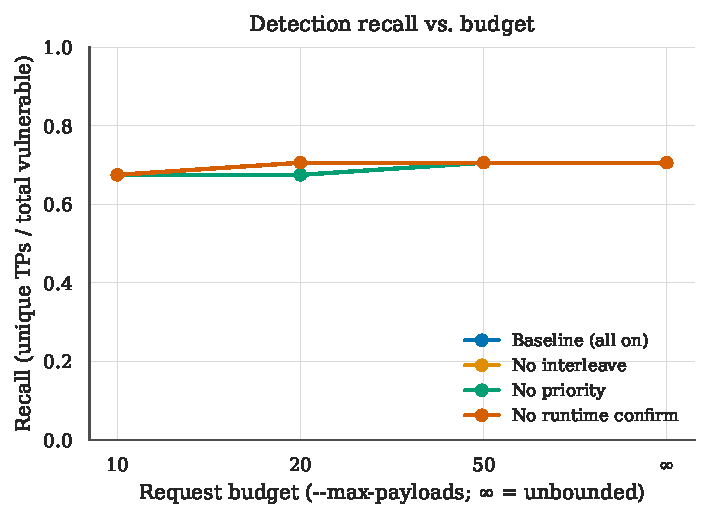
\includegraphics[width=\columnwidth]{fig1_detection_vs_budget.pdf}%
  }{%
    \fbox{\parbox[c][3.2cm][c]{0.9\columnwidth}{\centering\footnotesize
      \textsc{Placeholder} ---
      \code{figures/fig1\_detection\_vs\_budget.pdf}}}%
  }
  \caption{Recall (unique vulnerable instances detected $/$ total) as a
  function of the \code{-{}-max-payloads} request budget ($\infty$ =
  unbounded), one curve per pipeline configuration. The \code{baseline},
  \code{no-interleave}, \code{no-runtime-confirm}, and
  \code{no-adaptive-sorting} curves overlap.}
  \label{fig:deteccion-vs-presupuesto}
\end{figure}

\begin{figure}[t]
  \centering
  \IfFileExists{figures/fig2_ablation_impact.pdf}{%
    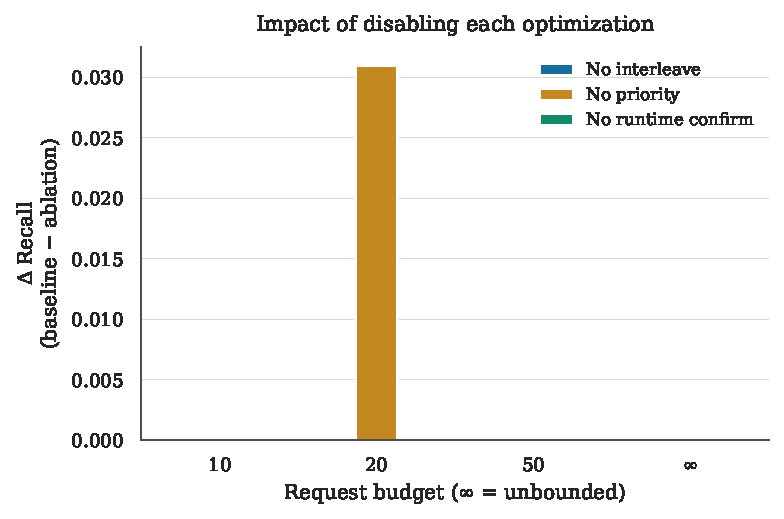
\includegraphics[width=\columnwidth]{fig2_ablation_impact.pdf}%
  }{%
    \fbox{\parbox[c][3.2cm][c]{0.9\columnwidth}{\centering\footnotesize
      \textsc{Placeholder} ---
      \code{figures/fig2\_ablation\_impact.pdf}}}%
  }
  \caption{Recall drop ($\text{baseline} - \text{ablation}$) from disabling
  each optimization, by budget. The only sizeable effect is
  \code{no-priority} at the \num{20}-request budget.}
  \label{fig:impacto-ablacion}
\end{figure}

\subsection{Metric summary and AUC}
\label{sec:res-auc}

At a budget of \num{20}~requests per parameter, \code{baseline} reaches a
detection-curve AUC of \ValorAUCBaseline{} (\cref{eq:auc}), with precision
\ValorPrecisionBaseline{}, recall \ValorRecallBaseline{}, and $F_1$
\ValorFOneBaseline{}, at a \ValorFPRBaseline{} false-positive rate
(\num{2} of \NumTrampas{}~traps). Disabling context interleaving, runtime
confirmation, or adaptive sorting leaves recall and AUC unchanged
(\ValorAUCNoInterleave{}, \ValorAUCNoRuntimeConfirm{}, and
\ValorAUCNoAdaptiveSorting{} respectively), but each trips one additional
known trap (FPR \ValorFPRBudgetAlto{}, \num{3} of \NumTrampas{}), fractionally
lowering precision to \num{63.7}\,\% and $F_1$ to \num{67.0}\,\% --- a
difference of a single false positive out of 210 findings. Disabling
prioritization is the only change with a practically visible cost: AUC drops
to \ValorAUCNoPriority{}, recall falls by \DeltaRecallNoPriority{}, and
precision by \DeltaPrecisionNoPriority{}, which in absolute terms amounts to
\NoPriorityVulnPerdidas{}~undetected vulnerabilities and
\NoPriorityFPnuevos{}~additional false positives relative to \code{baseline}.
At budgets \num{50} and $\infty$ the effect dissolves entirely: all five
configurations converge to \emph{identical} precision, recall
(\ValorRecallTecho{}), and $F_1$ (\cref{tab:auc}).

\begin{table}[t]
  \centering
  \caption{Per-run metrics and detection-curve AUC (\cref{eq:auc}). Source:
  \code{summary\_by\_run.csv}.}
  \label{tab:auc}
  \footnotesize
  \setlength{\tabcolsep}{4pt}
  \begin{tabular}{ll S[table-format=1.3] S[table-format=1.3] S[table-format=1.3] S[table-format=1.3]}
    \toprule
    Budget & Config. & {Prec.} & {Rec.} & {$F_1$} & {AUC} \\
    \midrule
    \multirow{5}{*}{10}
      & baseline           & 0.642 & 0.675 & 0.658 & 0.347 \\
      & no-interleave      & 0.642 & 0.675 & 0.658 & 0.347 \\
      & no-priority        & 0.642 & 0.675 & 0.658 & 0.348 \\
      & no-runtime-confirm & 0.649 & 0.675 & 0.662 & 0.351 \\
      & no-adaptive-sorting & 0.642 & 0.675 & 0.658 & 0.347 \\
    \midrule
    \multirow{5}{*}{20}
      & baseline           & 0.640 & 0.706 & 0.672 & 0.356 \\
      & no-interleave      & 0.637 & 0.706 & 0.670 & 0.356 \\
      & no-priority        & 0.585 & 0.675 & 0.627 & 0.350 \\
      & no-runtime-confirm & 0.637 & 0.706 & 0.670 & 0.355 \\
      & no-adaptive-sorting & 0.637 & 0.706 & 0.670 & 0.355 \\
    \midrule
    \multirow{5}{*}{50}
      & baseline           & 0.591 & 0.706 & 0.643 & 0.359 \\
      & no-interleave      & 0.591 & 0.706 & 0.643 & 0.366 \\
      & no-priority        & 0.591 & 0.706 & 0.643 & 0.360 \\
      & no-runtime-confirm & 0.591 & 0.706 & 0.643 & 0.359 \\
      & no-adaptive-sorting & 0.591 & 0.706 & 0.643 & 0.366 \\
    \midrule
    \multirow{5}{*}{$\infty$}
      & baseline           & 0.591 & 0.706 & 0.643 & 0.369 \\
      & no-interleave      & 0.591 & 0.706 & 0.643 & 0.369 \\
      & no-priority        & 0.591 & 0.706 & 0.643 & 0.369 \\
      & no-runtime-confirm & 0.591 & 0.706 & 0.643 & 0.369 \\
      & no-adaptive-sorting & 0.591 & 0.706 & 0.643 & 0.369 \\
    \bottomrule
  \end{tabular}
\end{table}

\subsection{Statistical significance}
\label{sec:res-stats}

Over the per-instance detection-cost vectors (pooled block across the
\NumBloquesCompletos{}~complete budgets, $n = \ValorFriedmanN{}$), the
Friedman test rejects the equivalence of the four configurations
($\chi^2 = \ValorFriedmanChiSq{}$, $p = \ValorFriedmanP{}$). However, the
effect size is \emph{negligible} in the pairwise \code{baseline}-versus-ablation
comparisons: Cliff's $\delta$ of \ValorCliffNoInterleave{}
(\code{no-interleave}), \ValorCliffNoPriority{} (\code{no-priority}), and
\ValorCliffNoRuntimeConfirm{} (\code{no-runtime-confirm}), all with
$\lvert\delta\rvert < \num{0.02}$ (\cref{tab:stats}). The fifth arm,
\code{no-adaptive-sorting}, is analyzed separately in
\cref{sec:res-adaptive}. The Nemenyi post-hoc
fails to separate \code{no-runtime-confirm} from \code{baseline}
($p = \ValorNemenyiNoRuntimeConfirm{}$). The reading is that the differences
Friedman detects are of \emph{fine-grained request ordering} ---
statistically real given the large number of blocks, but with no practical
translation into the final detected set. The only operationally consequential
change is the loss of selectivity of \code{no-priority} under tight budgets,
already described in \cref{sec:res-auc}; note that \code{no-priority} even
lowers the mean detection cost (\ValorCosteBaseline{} $\to$
\ValorCosteNoPriority{} requests), i.e., it hits earlier on average but at the
cost of precision.

\begin{table}[t]
  \centering
  \caption{Tests on per-instance detection cost, \code{baseline} versus each
  ablation (pooled block, $n = \ValorFriedmanN{}$). Wilcoxon with
  Benjamini--Hochberg correction; $p_{\text{Nem.}}$ from the Nemenyi post-hoc;
  Cliff's $\delta$ as effect size. Source: \code{stats.json}.}
  \label{tab:stats}
  \footnotesize
  \setlength{\tabcolsep}{4pt}
  \resizebox{\columnwidth}{!}{%
  \begin{tabular}{lccccl}
    \toprule
    \code{baseline} vs & Mean cost & $p_{\text{BH}}$ & $p_{\text{Nem.}}$
      & Cliff's $\delta$ & Magnitude \\
    \midrule
    no-interleave      & \ValorCosteBaseline{}$\to$\ValorCosteNoInterleave{} & \ValorWilcoxonPNoInterleave{}
      & \ValorNemenyiNoInterleave{} & \ValorCliffNoInterleave{}
      & \MagnitudCliffNoInterleave{} \\
    no-priority        & \ValorCosteBaseline{}$\to$\ValorCosteNoPriority{} & \ValorWilcoxonPNoPriority{}
      & \ValorNemenyiNoPriority{} & \ValorCliffNoPriority{}
      & \MagnitudCliffNoPriority{} \\
    no-runtime-confirm & \ValorCosteBaseline{}$\to$\ValorCosteNoRuntimeConfirm{} & \ValorWilcoxonPNoRuntimeConfirm{}
      & \ValorNemenyiNoRuntimeConfirm{} & \ValorCliffNoRuntimeConfirm{}
      & \MagnitudCliffNoRuntimeConfirm{} \\
    \bottomrule
  \end{tabular}}
  \\[2pt]
  \footnotesize\emph{Global Friedman: $\chi^2 = \ValorFriedmanChiSq{}$,
  $p = \ValorFriedmanP{}$.}
\end{table}

\subsection{Critical-difference diagram}
\label{sec:res-cd}

\Cref{fig:cd} ranks the four Friedman-tested configurations by mean
detection-cost rank
(pooled block, $n = \ValorFriedmanN{}$). The Nemenyi post-hoc leaves only
\code{baseline} and \code{no-runtime-confirm} unseparated (horizontal bar);
\code{no-interleave} sits at the worst rank (latest detection) and
\code{no-priority} at the best. This last point must be read carefully:
\code{no-priority} advances the mean first detection because it tries
apparently high-yield trivial payloads first, but ---as \cref{tab:auc}
shows--- it does so at the cost of \NoPriorityVulnPerdidas{}~vulnerabilities
and \NoPriorityFPnuevos{}~false positives. The diagram compares \emph{when}
each configuration detects, not \emph{how much} nor at what precision.

\begin{figure}[t]
  \centering
  \IfFileExists{figures/fig3_cd_diagram.pdf}{%
    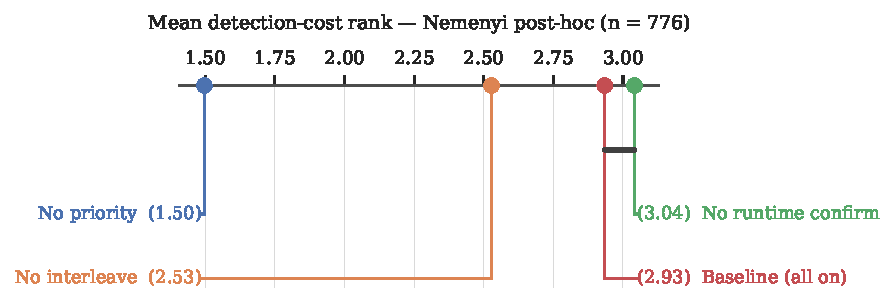
\includegraphics[width=\columnwidth]{fig3_cd_diagram.pdf}%
  }{%
    \fbox{\parbox[c][2.6cm][c]{0.9\columnwidth}{\centering\footnotesize
      \textsc{Pending} --- \code{figures/fig3\_cd\_diagram.pdf}.}}%
  }
  \caption{Critical-difference diagram (Nemenyi post-hoc, $\alpha = 0.05$) on
  mean rank of per-instance detection cost. Lower rank $=$ earlier detection.
  Configurations joined by a horizontal bar are not distinguishable. Since all
  effect sizes are negligible (\cref{tab:stats}), the diagram is indicative of
  ordering, not of a practical advantage.}
  \label{fig:cd}
\end{figure}

\subsection{Adaptive sorting: live feedback versus static a-priori order}
\label{sec:res-adaptive}

\Cref{fig:first-tp-ecdf} contrasts the per-instance first-true-positive
request cost between \code{baseline} (live adaptive sorting) and
\code{no-adaptive-sorting} (static a-priori order), pooled across budgets.
The paired Wilcoxon test and Cliff's $\delta$ (\cref{sec:tests}) quantify
whether re-ranking the queue mid-scan from observed hit/miss feedback shifts
first-detection cost relative to committing to the \code{freq} order fixed
before the scan starts.

\begin{figure}[t]
  \centering
  \IfFileExists{figures/fig4_first_tp_ecdf.pdf}{%
    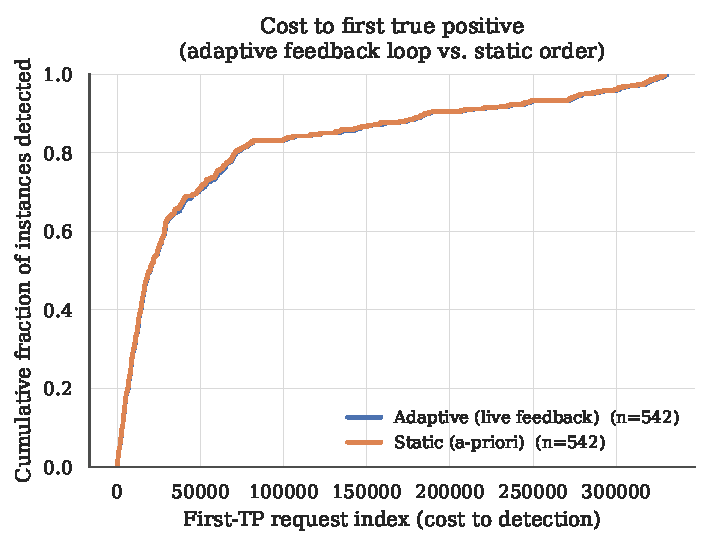
\includegraphics[width=\columnwidth]{fig4_first_tp_ecdf.pdf}%
  }{%
    \fbox{\parbox[c][2.6cm][c]{0.9\columnwidth}{\centering\footnotesize
      \textsc{Pending} --- \code{figures/fig4\_first\_tp\_ecdf.pdf}.}}%
  }
  \caption{ECDF of the per-instance first-true-positive request index:
  adaptive (\code{baseline}) versus static a-priori order
  (\code{no-adaptive-sorting}), pooled across budgets.}
  \label{fig:first-tp-ecdf}
\end{figure}

\subsection{External baseline: OWASP ZAP on the same target list}
\label{sec:res-external}

To ground \code{baseline} against an external scanner rather than only
against its own disabled stages, we ran OWASP ZAP 2.17.0 (default
active-scan policy, default attack strength and alert threshold) against the
identical \num{338}-target list, one URL-scoped active scan per target
(\code{recurse=false}), graded by the same independent oracle against the
same ground truth. \Cref{tab:zap} reports the result, both over every alert
ZAP raised (\emph{unrestricted}) and restricted to the five vulnerability
categories this ground truth actually scores --- \code{SQLInjection},
\code{XSS}, \code{PathTraversal}, \code{CommandInjection}, and
\code{LDAPInjection} --- since ZAP's default policy also reports categories
(missing security headers, cookie flags, CSP configuration, \ldots) that
\herramienta's testers do not attempt and that consequently have no
population to be scored against in this ground truth.

\begin{table}[t]
  \centering
  \caption{OWASP ZAP 2.17.0 versus \herramienta's \code{baseline}, same
  \num{338}-target list, same oracle. ZAP's \emph{restricted} column drops
  alert categories outside this ground truth's five scored types. Source:
  \code{tools/run\_zap\_baseline.py}.}
  \label{tab:zap}
  \footnotesize
  \setlength{\tabcolsep}{4pt}
  \begin{tabular}{lccccc}
    \toprule
    & {Prec.} & {Rec.} & {$F_1$} & {FPR} & {Wall-clock} \\
    \midrule
    ZAP (unrestricted) & 0.252 & 0.706 & 0.371 & 0.000 & \SI{1961}{\second} \\
    ZAP (restricted)   & 0.890 & 0.706 & 0.787 & 0.000 & \SI{1961}{\second} \\
    \herramienta\ (budget 20)  & 0.640 & 0.706 & 0.672 & 0.014 & \SI{183}{\second} \\
    \herramienta\ (budget $\infty$) & 0.591 & 0.706 & 0.643 & 0.021 & \SI{1609}{\second} \\
    \bottomrule
  \end{tabular}
\end{table}

Three results are worth stating plainly, including the ones that do not
favor \herramienta. First, \textbf{recall is identical}: ZAP and
\code{baseline} both detect exactly \num{137} of the \num{194} vulnerable
instances, at every budget --- the same subset, since both tools' misses are
concentrated in the same harder categories. This is independent evidence for
this paper's central claim about the target, not the tool: OWASP Benchmark's
\num{57} undetected instances resist a second, independently engineered
scanner just as they resist this one, which is far more consistent with a
property of the benchmark than of either tool. Second, \textbf{ZAP's FPR on
this run is \num{0}\,\%} (zero trap hits out of \num{144}) versus
\code{baseline}'s \ValorFPRBaseline{}--\ValorFPRBudgetAlto{}: on the specific
\num{144} known-safe traps in this ground truth, ZAP's default policy is
strictly more conservative than \herramienta's heuristic confirmation stage.
Third, \textbf{restricted precision favors ZAP}, but the comparison is
apples-to-oranges by construction: ZAP's default policy is a general-purpose
scanner run unfiltered, while \code{baseline} tests only the five categories
this ground truth scores, so \emph{restricted} precision --- computed after
manually filtering ZAP down to the same five categories --- necessarily
flatters ZAP relative to its own unfiltered, real-world operating point. Read
this row as a best-case number for ZAP, not a fair head-to-head: restricted
precision is \num{89.0}\,\% versus \ValorPrecisionBaseline{} for
\code{baseline} at budget \num{20}, while ZAP's actual out-of-the-box
(\emph{unrestricted}) precision is \num{25.2}\,\%, since its default policy
reports \num{582} raw alerts across every category it tests, only \num{154} of which
fall inside this ground truth's five scored types. The wall-clock gap is
large in the other direction: ZAP's default active scan takes
\SI{1961}{\second} for these \num{338} targets, comparable to
\herramienta's \emph{unbounded}-budget run rather than its saturating
\num{20}-request budget, which reaches the same recall in
\SI{183}{\second} --- roughly \num{11}$\times$ faster at the budget where
\code{baseline} already saturates (\cref{sec:res-eficiencia}).

This is a single run of each tool, not a repeated-trials comparison, and the
two scanners' default policies test different rule sets by design (ZAP's is
far broader), so \cref{tab:zap} should be read as one honest data point,
not a leaderboard result. Potti~\emph{et al.} independently report OWASP ZAP
v2.12.0/v2.13.0 aggregate results on the full OWASP Benchmark project (all
vector types, not just \code{GET}) of \num{68.75}--\num{74.63}\,\% recall at
\num{0.86}--\num{3.45}\,\% FPR~\cite{potti2025benchmarking}; our
single-run, \code{GET}-only, ZAP-2.17.0 result of \num{70.6}\,\%
recall at \num{0}\,\% FPR is consistent with that range.

\subsection{Summary of findings}
\label{sec:res-sintesis}

\begin{enumerate}
  \item The \code{baseline} pipeline saturates at \ValorRecallTecho{} recall
  and \ValorFPRBaseline{} FPR with only \num{20}~requests per parameter;
  widening the budget further adds no detection, only false positives
  (precision drops from \ValorPrecisionBaseline{} to \num{59.1}\,\% between
  the \num{20} and $\infty$ budgets).
  \item \textbf{Confidence-based prioritization} is the only stage whose
  removal has a measurable cost, and it concentrates at tight budgets:
  $-\DeltaRecallNoPriority{}$ recall and $-\DeltaPrecisionNoPriority{}$
  precision at budget \num{20}, an effect that disappears from \num{50}
  onward.
  \item \textbf{Context interleaving}, \textbf{runtime confirmation}, and
  \textbf{live adaptive sorting} do not change recall, precision, or FPR on
  this benchmark; their effect on request order is statistically detectable
  but negligible in magnitude.
  \item Consequently, the value of payload scheduling in this scenario is one
  of \emph{anticipation} (higher AUC under a tight budget), not of a higher
  detection \emph{ceiling}.
\end{enumerate}

%% 04b_ai_triage.tex — Evaluación del triaje basado en LLM.
%%
%% Contenido numérico: testbed/experiment_results.csv (filas ai-triage) +
%% testbed/analysis/ai_triage.json, generado por tools/analyze_results.py.

\section{LLM-Based Triage Evaluation}
\label{sec:ai-triage}

Beyond the scheduling pipeline, \herramienta offers an opt-in LLM-based
triage stage (\code{-{}-enable-ai-triaging}) that re-scores every raw finding
using the request/response evidence already collected by the heuristic
engine, without an additional network round trip to the target. Each
candidate finding is sent to an LLM backend (\code{AgentClient}) together
with its payload, response snippet, and heuristic confidence; the model
returns a suppression probability, and findings scoring above
\code{ai\_fp\_threshold} ($=\num{0.75}$ by default) are dropped before the
report is written. Degradation is transparent: if \code{ai\_module} is
unavailable, the backend fails its health check, or a per-call request
errors, the tester falls back to the deterministic heuristic decision and the
scan continues.

\subsection{Setup}

The \code{ai-triage} arm layers this stage on top of \code{baseline} ---
identical scheduling pipeline, identical corpus, identical budgets --- so any
difference against \code{baseline} isolates the triage stage's effect.
\Cref{tab:aitriage} reports, per budget: the number of candidates the model
triaged (\code{AI\_Triaged}), how many it suppressed
(\code{AI\_Suppressed}), how many of those were true false positives
(\code{AI\_FP\_Suppressed}), and how many were real vulnerabilities the model
incorrectly hid (\code{AI\_FN\_Introduced}).

\begin{table}[t]
  \centering
  \caption{LLM triage audit trail, \code{ai-triage} arm (\code{baseline}
  pipeline + LLM-based triage, \code{ai\_fp\_threshold}$=\num{0.75}$). Source:
  \code{experiment\_results.csv}.}
  \label{tab:aitriage}
  \footnotesize
  \setlength{\tabcolsep}{4pt}
  \begin{tabular}{r S[table-format=3.0] S[table-format=2.0] S[table-format=2.0] S[table-format=2.0]}
    \toprule
    Budget & {Triaged} & {Suppr.} & {FP suppr.} & {FN introd.} \\
    \midrule
    10        & 441 & 0 & 0 & 0 \\
    20        & 459 & 0 & 0 & 0 \\
    50        & \ValorAITriageBudgetFiftyTriaged{} & \ValorAITriageBudgetFiftySuppressed{}
              & \ValorAITriageBudgetFiftyFPSuppressed{} & \ValorAITriageBudgetFiftyFNIntroduced{} \\
    $\infty$  & \ValorAITriageBudgetInfTriaged{} & \ValorAITriageBudgetInfSuppressed{}
              & \ValorAITriageBudgetInfFPSuppressed{} & \ValorAITriageBudgetInfFNIntroduced{} \\
    \bottomrule
  \end{tabular}
\end{table}

\subsection{Latency overhead}
\label{sec:ai-triage-latency}

Triage calls run through a \code{BatchingTriageClient} that queues candidates
and issues them off the event loop, overlapped with the scan's own in-flight
requests, rather than blocking on a round trip per finding. Comparing the
wall-clock span of each \code{ai-triage} run against its \code{baseline}
counterpart at the same budget (identical telemetry row count, so identical
work) isolates the added cost: \SI{+12.2}{\second} at budget \num{10},
\SI{-32.2}{\second} at budget \num{20}, \SI{+0.6}{\second} at budget
\num{50}, and \SI{-41.3}{\second} at budget $\infty$ (a \SI{1568}{\second}
run) --- within ordinary run-to-run variance in both directions, not a
systematic overhead. This does not mean LLM inference is free: it means the
async batching design keeps its latency off the scan's critical path for
this backend and candidate volume (\ValorAITriageTotalTriaged{} candidates
across four runs). A backend with materially higher per-call latency, or a
target with a much larger candidate volume, could still saturate the batching
queue; that stress case is not exercised here.

\subsection{Result: null suppression under the default threshold}
\label{sec:ai-triage-result}

Across every evaluated budget, the LLM triage stage suppressed
\textbf{zero} findings: \ValorAITriageTotalTriaged{} candidates were sent to
the model and none scored above the \num{0.75} suppression threshold. As a
direct consequence, \code{ai-triage} precision, recall, and $F_1$ are
identical to \code{baseline}'s at every budget (\cref{tab:auc} versus
\cref{tab:aitriage}), and no false negative was introduced.

This is a legitimate negative result, not an inconclusive one, and it is
consistent with the same root cause identified in the scheduling ablation
(\cref{sec:res-sintesis}): OWASP Benchmark's trigger signals are unusually
regular. Its reflected-XSS and error-based-SQLi findings carry unambiguous
textual evidence (the payload verbatim in the response, or a
database-specific error string), which is exactly the kind of signal a
threshold-\num{0.75} triage model is calibrated \emph{not} to override,
since doing so risks the false negative the related-work literature
identifies as the real cost of aggressive
triage~\cite{du2026reducing,ameen2026qasecclaw}. On this benchmark the
already-low false-positive population (\NumTrampas{} known traps, a
\ValorFPRBaseline{} FPR at \code{baseline}) leaves little genuine noise for
an LLM triage stage to remove: the reported 88--98\,\% false-positive
reductions in the static-analysis
literature~\cite{munson2025llmfriends,ameen2026qasecclaw,du2026reducing} are
measured against corpora with a substantially higher false-positive rate than
the one this DAST pipeline already achieves through its heuristic
confirmation stage (\cref{sec:confirmacion}) before triage ever runs: this
benchmark is close to the wrong instrument for the question the stage is
meant to answer, and a null suppression rate here is evidence about the
target, not a validation of the triage stage's safety or effectiveness in
general. We report it anyway, instead of omitting an inconvenient arm, because
the alternative --- silently dropping the evaluation --- would be worse
scientific practice than an honest negative result. Whether the stage
suppresses real noise, and at what recall cost, on a target with a
deliberately elevated false-positive rate is the open question the future
work of \cref{sec:conclusion} takes up.

%% 05_amenazas_validez.tex — Validez interna, externa y de constructo.

\section{Threats to Validity}
\label{sec:amenazas}

\subsection{Internal validity: JVM warm-up and isolation}

OWASP Benchmark is a Java application on a servlet container. The JVM's JIT
compiler optimizes hot code paths after several invocations, so the first
requests to an endpoint are systematically slower than later ones. This
introduces two biases: (i)~the time-based confirmation stage
(\cref{sec:confirmacion}) could interpret warm-up latency as a
payload-induced delay, inflating \textsc{confirmed} findings in the early
phases of the scan; and (ii)~the detection-cost metric is measured in request
index, not time, so it is robust to warm-up, but comparing absolute latency
across configurations is not.

Mitigations applied: baseline latency is resampled immediately before every
timed test (not once at the start); the threshold $\tau = \SI{4}{\second}$ is
generous relative to the observed warm-up variance; and every configuration
runs against the same freshly started container, with a single client and no
concurrent traffic, so any residual warm-up bias is common to every arm and
cancels out in the paired contrast. Resource isolation (dedicated container,
local network, no other scanners) reduces run-to-run variance, but does not
eliminate that introduced by the OS scheduler or JVM garbage collection. A
replication with explicit warm-up ($N$ discard requests per endpoint) remains
future work.

\subsection{External validity: restriction to \code{GET} vectors}

The study is limited to \num{338}~injection points in \code{GET} query
parameters, each saturating at \num{20}~requests. This corpus is too small
to exercise the combinatorial explosion motivating
\cref{sec:intro}'s architecture; the ablation demonstrates the scheduling
mechanics work correctly under a modest, saturating budget, not that they
scale favorably against a payload space large enough to actually explode.
\code{POST} vectors with an
\code{application/x-www-form-urlencoded} or JSON body, headers, cookies, and
path parameters are out of scope. Consequently, the recall and cost results
do \emph{not} generalize directly to the full attack surface of a real
application: categories with higher incidence in \code{POST} bodies (e.g.,
SQL injection in authentication forms) are under-represented. In addition,
OWASP Benchmark is a synthetic testbed; its trigger payloads and response
patterns are more regular than those of production applications, which likely
overestimates any scanner's absolute
recall~\cite{doupe2010johnny}. The contribution that does hold under this
restriction is the \emph{relative} one: the effect of each pipeline stage on a
homogeneous, controlled target set.

The cross-tool comparison in \cref{sec:res-external} is a single run of each
tool, not repeated trials, and the two scanners' default policies test
different, non-identical rule sets by design; a single run cannot rule out
run-to-run variance on either side, and the \emph{unrestricted} precision
comparison in particular conflates ``did not report this category'' with
``reported it incorrectly'' for whichever scanner's default policy is
narrower in scope. Readers should treat \cref{tab:zap} as one honest data
point, not a leaderboard result generalizing to other targets, policies, or
tool versions.

\subsection{Construct and conclusion validity}

The oracle collapses type aliases onto common buckets; a detection with the
``correct'' type but the ``wrong'' subclass (e.g., \emph{blind} versus
\emph{error-based}) counts as a hit. FPR is defined only over the
\num{144}~explicit traps; false positives against tuples that ground truth
does not mention have no reference population and are not scored. Finally, the
number of blocks per budget is bounded by $\lvert P \rvert = 194$, sufficient
for the Friedman test but modest for the Nemenyi post-hoc; critical-difference
diagrams are interpreted as indicative rather than conclusive.

The LLM-triage evaluation (\cref{sec:ai-triage}) carries an additional threat:
the backend model, prompt, and \code{ai\_fp\_threshold} are fixed at their
defaults for a single provider; the null suppression rate reported there is a
property of that specific configuration on this benchmark, not a general
claim about LLM-based triage.

%% 06_conclusion.tex — Conclusión y trabajo futuro.

\section{Conclusion and Future Work}
\label{sec:conclusion}

We presented \herramienta, an asynchronous DAST engine whose architecture
explicitly separates payload scheduling and finding confirmation into
decoupled stages, together with a reproducible evaluation methodology on
OWASP Benchmark, an independent oracle, an RCBD design, and a
corpus-hashing manifest.

The ablation study yields a nuanced result. Over the \NumObjetivos{}
\code{GET}-parameter targets, the full heuristic pipeline reaches
\ValorRecallTecho{} recall at \ValorFPRBaseline{} FPR, and \emph{saturates}
already at \num{20}~requests per parameter. Of the four scheduling
optimizations evaluated, only \textbf{confidence-based prioritization}
produces a practically consequential change, and it is bounded to tight
budgets: disabling it costs \DeltaRecallNoPriority{} recall and
\DeltaPrecisionNoPriority{} precision at budget \num{20}, and nothing from
\num{50} onward. \textbf{Context interleaving}, \textbf{runtime
confirmation}, and \textbf{live adaptive sorting} do not change recall,
precision, or FPR on this benchmark; the Friedman test detects differences in
request \emph{order} ($p = \ValorFriedmanP{}$), but with negligible effect
sizes ($\lvert\delta\rvert < \num{0.02}$). Layering \textbf{LLM-based triage}
on top of the baseline pipeline suppressed no findings at any of the four
evaluated budgets under the default confidence threshold, at no measured
wall-clock cost (\cref{sec:ai-triage}) ---
consistent with the same underlying explanation as the scheduling ablation:
OWASP Benchmark's trigger signals are regular enough that a conservative
triage model finds nothing it is confident enough to drop. The operational
conclusion is that, on a benchmark with trigger signals as regular as OWASP
Benchmark's, the benefit of payload scheduling is one of \emph{anticipation}
--- higher area under the detection curve when the budget is tight --- rather
than a higher detection \emph{ceiling}, and that neither runtime confirmation
nor LLM triage penalize precision because the raw indicators are already
reliable in this scenario.

\noindent\textbf{Future work.}
\begin{enumerate}
  \item Repeat the external baseline of \cref{sec:res-external} with
  multiple trials of OWASP ZAP (and add Burp Suite and/or Nuclei) to turn the
  current single-run comparison into a statistically tested one, and restrict
  each tool's active-scan policy to a matched rule set for a stricter
  apples-to-apples reading.
  \item Repeat the study on real-world applications and benchmarks with noisy
  signals, where runtime confirmation and LLM-based triage should show the
  false-positive-reduction value that was not observable here.
  \item Extend the benchmark to \code{POST} vectors, headers, and cookies to
  characterize categories that are currently under-represented.
  \item Widen the grid to budgets $\le \num{10}$ with replicates, where the
  effect of prioritization is largest, to narrow the confidence intervals.
  \item Add explicit JVM warm-up and repeat the absolute-latency analysis
  across configurations.
  \item Sweep the LLM triage confidence threshold and backend model, and
  evaluate triage on a corpus with a deliberately elevated false-positive
  rate to characterize the suppression/false-negative trade-off this
  benchmark could not exercise.
  \item Publish the complete set of manifests and JSONL traces as a
  verifiable research artifact.
  \item Extend the engine into the autonomous red-team pipeline currently
  under development in this repository --- a LangGraph orchestrator
  coordinating attacker, adaptive-fuzzer, CTI-ingestion, and reporting agents
  on top of \herramienta's scanning core --- and evaluate it as its own
  experimental subject once it reaches a stable interface.
\end{enumerate}


% ---------------------------------------------------------------------------
\section*{Artifact Availability}
The tool's source code, the ground-truth generator, the experiment
orchestrator, the grading oracle, and the analysis scripts are distributed
with the project repository. Every reported run ships its own reproducibility
manifest (\cref{sec:manifiesto}).

% ---------------------------------------------------------------------------
\bibliographystyle{IEEEtran}
\bibliography{refs}

\end{document}
